%\subsection{تخمین پارامترهای کانال پپچ}
%برای اصلاح پارامترهای پپچ چندین آزمایش انجام شد و با استفاده از داده‌های ثبت شده از وضعیت استند در کانال پپچ و جعبه‌ابزار
%\lr{Parameter Estimator}،
%پارامترهای کانال پپچ اصلاح شدند.
%برای انجام آزمایش هر یک از موتورهای دو و چهار  با دور مختلف شروع به حرکت کردند و از خروجی سنسور داده برداری شد. سپس، مدل و داده‌های ثبت شده‌ی سنسور (وضعیت استند در کانال پپچ) به جعبه‌ابزار
%\lr{Parameter Estimator}
%داده‌شد. وضعیت کانال پپچ استند در شبیه‌سازی و واقعیت بعد از اصلاح پارامترهای کانال پپچ در شکل‌های
%\ref{pitch_ps1}, \ref{pitch_ps2}, و \ref{pitch_ps3}
%مقایسه شده است.


لازم به ذکر است، برای اصلاح سایر پارامترهای کانال رول، پارامترهای اصلاح شده در بخش بالا ثابت در نظر گرفته شده‌است.



\begin{minipage}[H]{\linewidth}
	\hfill
	\begin{minipage}[b]{0.49\linewidth}
		\centering
		\begin{tabular}{ccc}\hline
			پارامتر & مقدار اولیه  & مقدار بعد از اصلاح
			\\ \hline
			$B_3$  & $1.1\times10^{-4}$ & $7.13\times10^{-5}$ \\ \hline
			\\
			\\\\\\
		\end{tabular}
	\captionsetup{justification=centering}
		\captionof{table}{مقايسه پارامترهای کانال پیچ قبل و بعد از اصلاح}
	\end{minipage}
	\begin{minipage}[b]{0.48\linewidth}
		\centering
		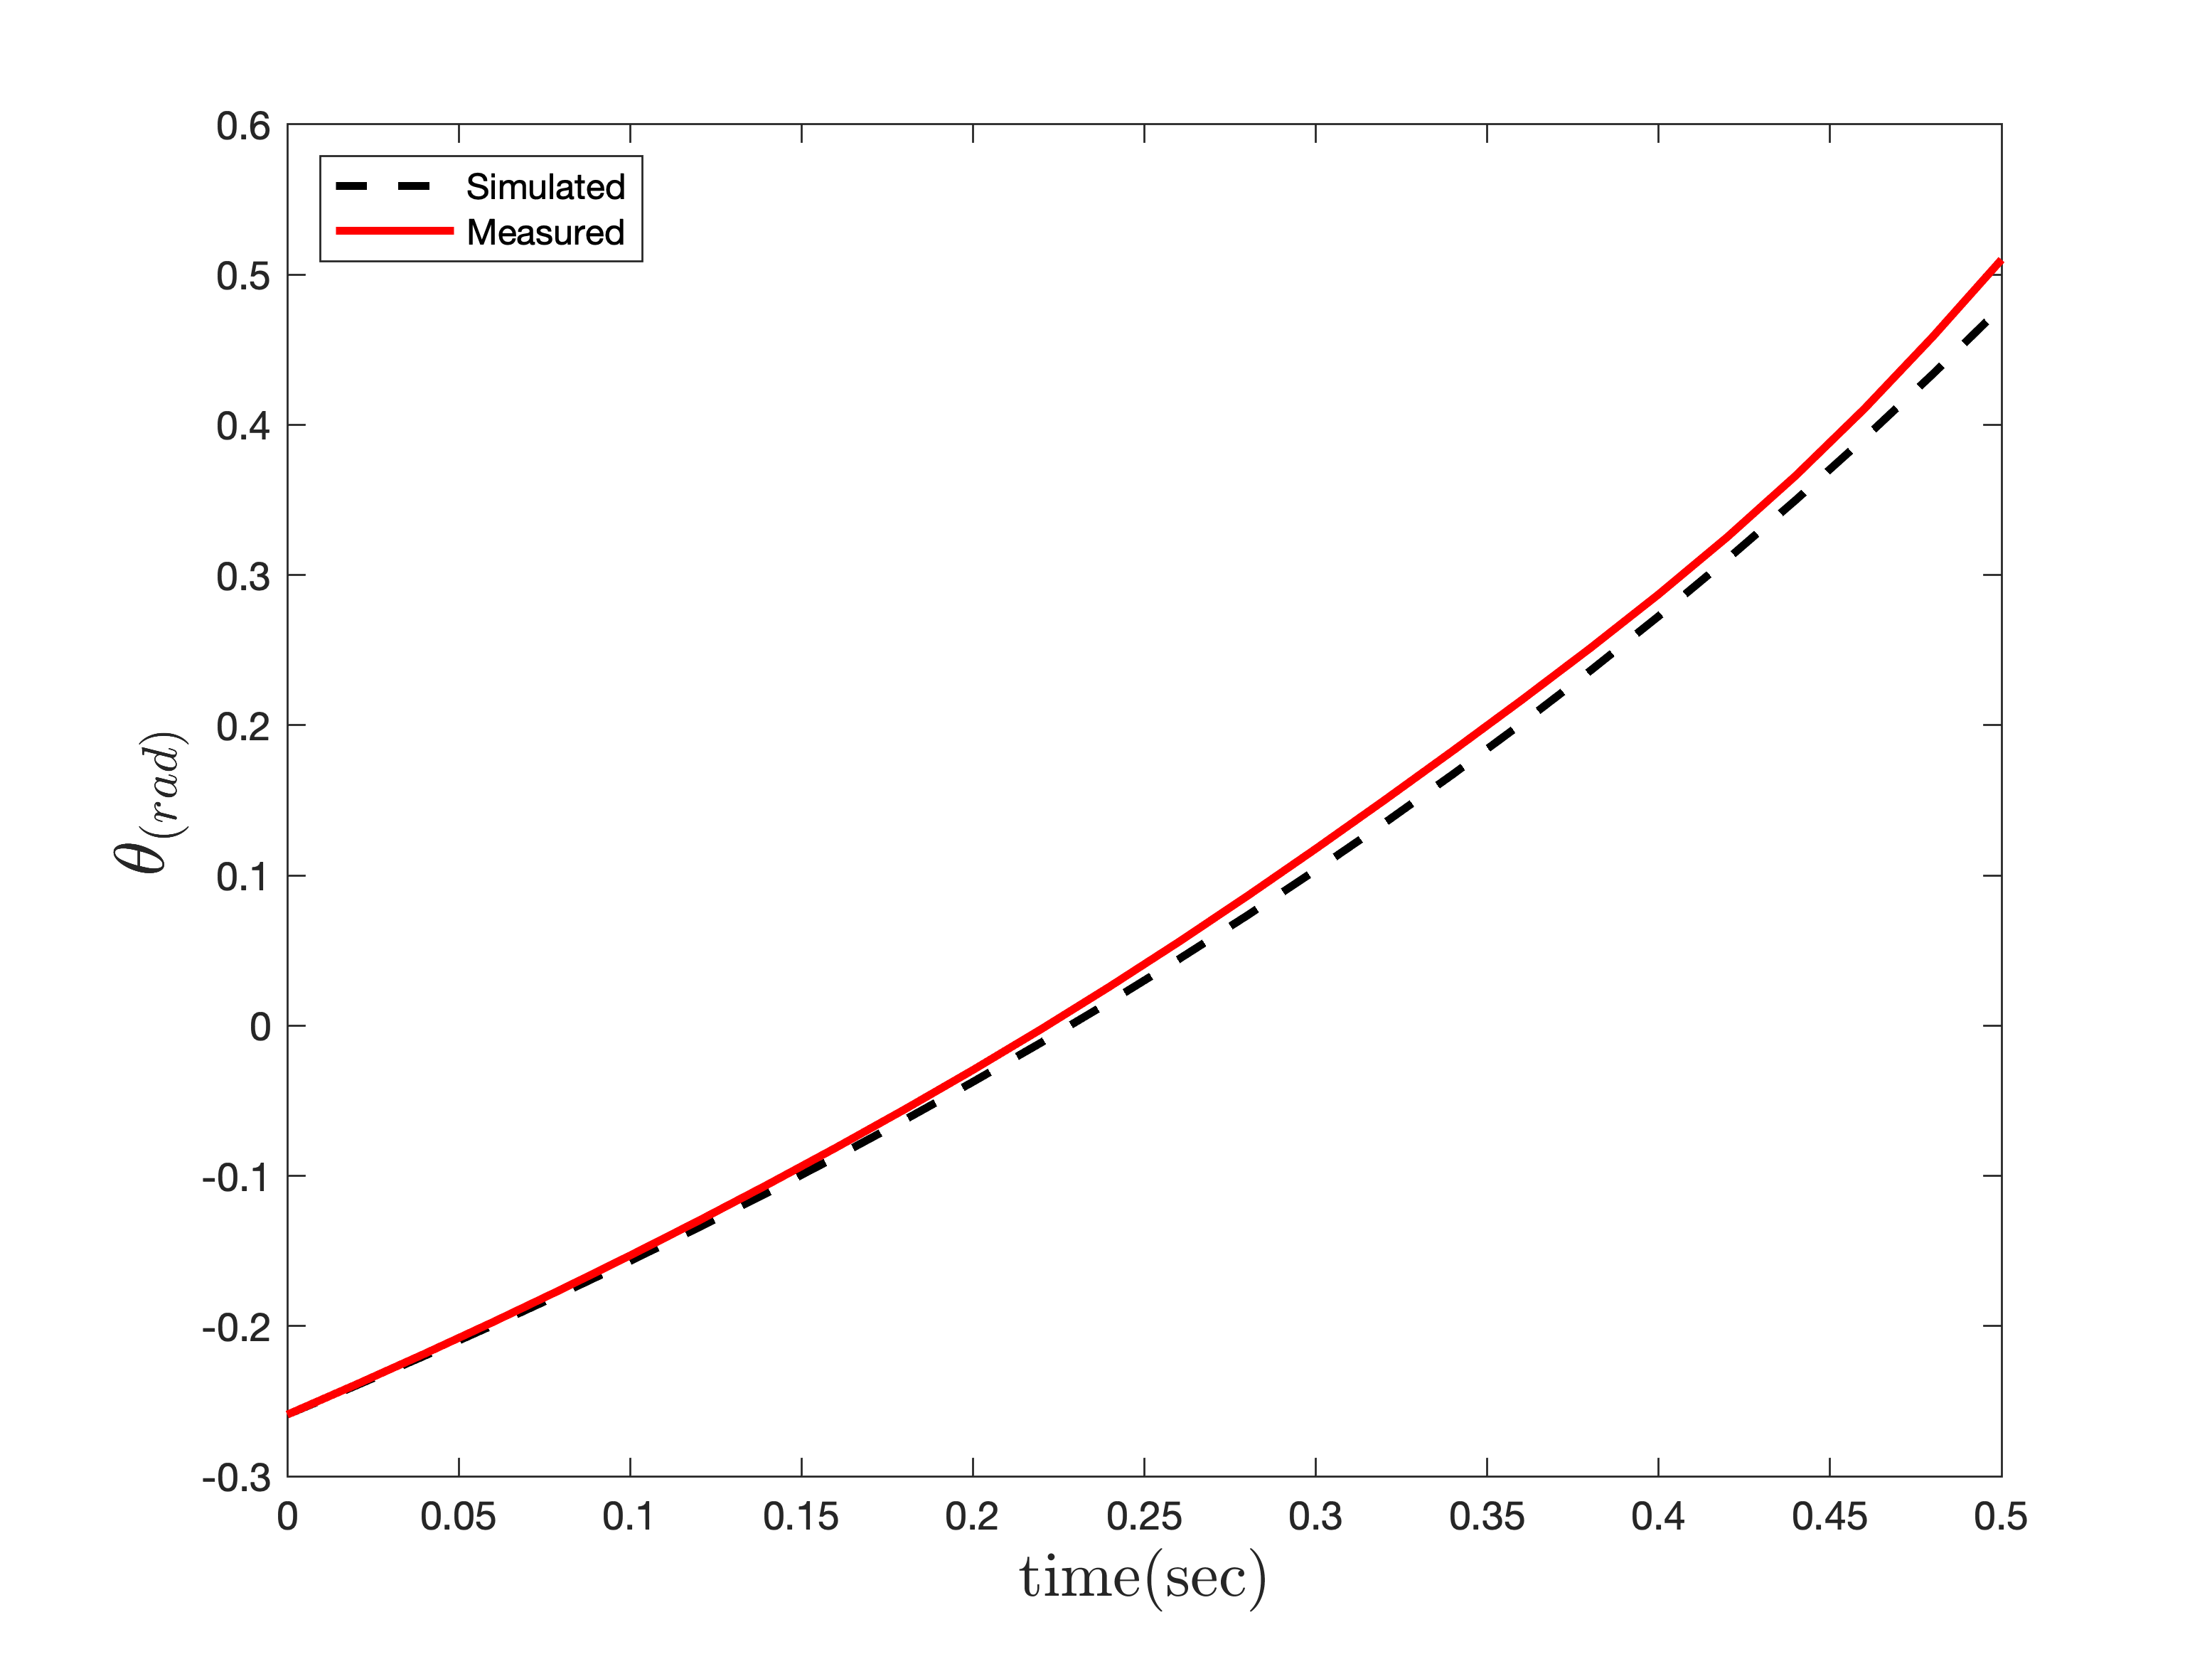
\includegraphics[width=1\linewidth]{../Figures/RCP/pitch_parameter_estimation/RCP_pitch_S1.png}
		\captionsetup{justification=centering}
		\captionof{figure}{مقايسه وضعیت کانال پیچ در شبیه‌سازی و واقعیت}
	\end{minipage}
\end{minipage}



%\begin{figure}[H]
%	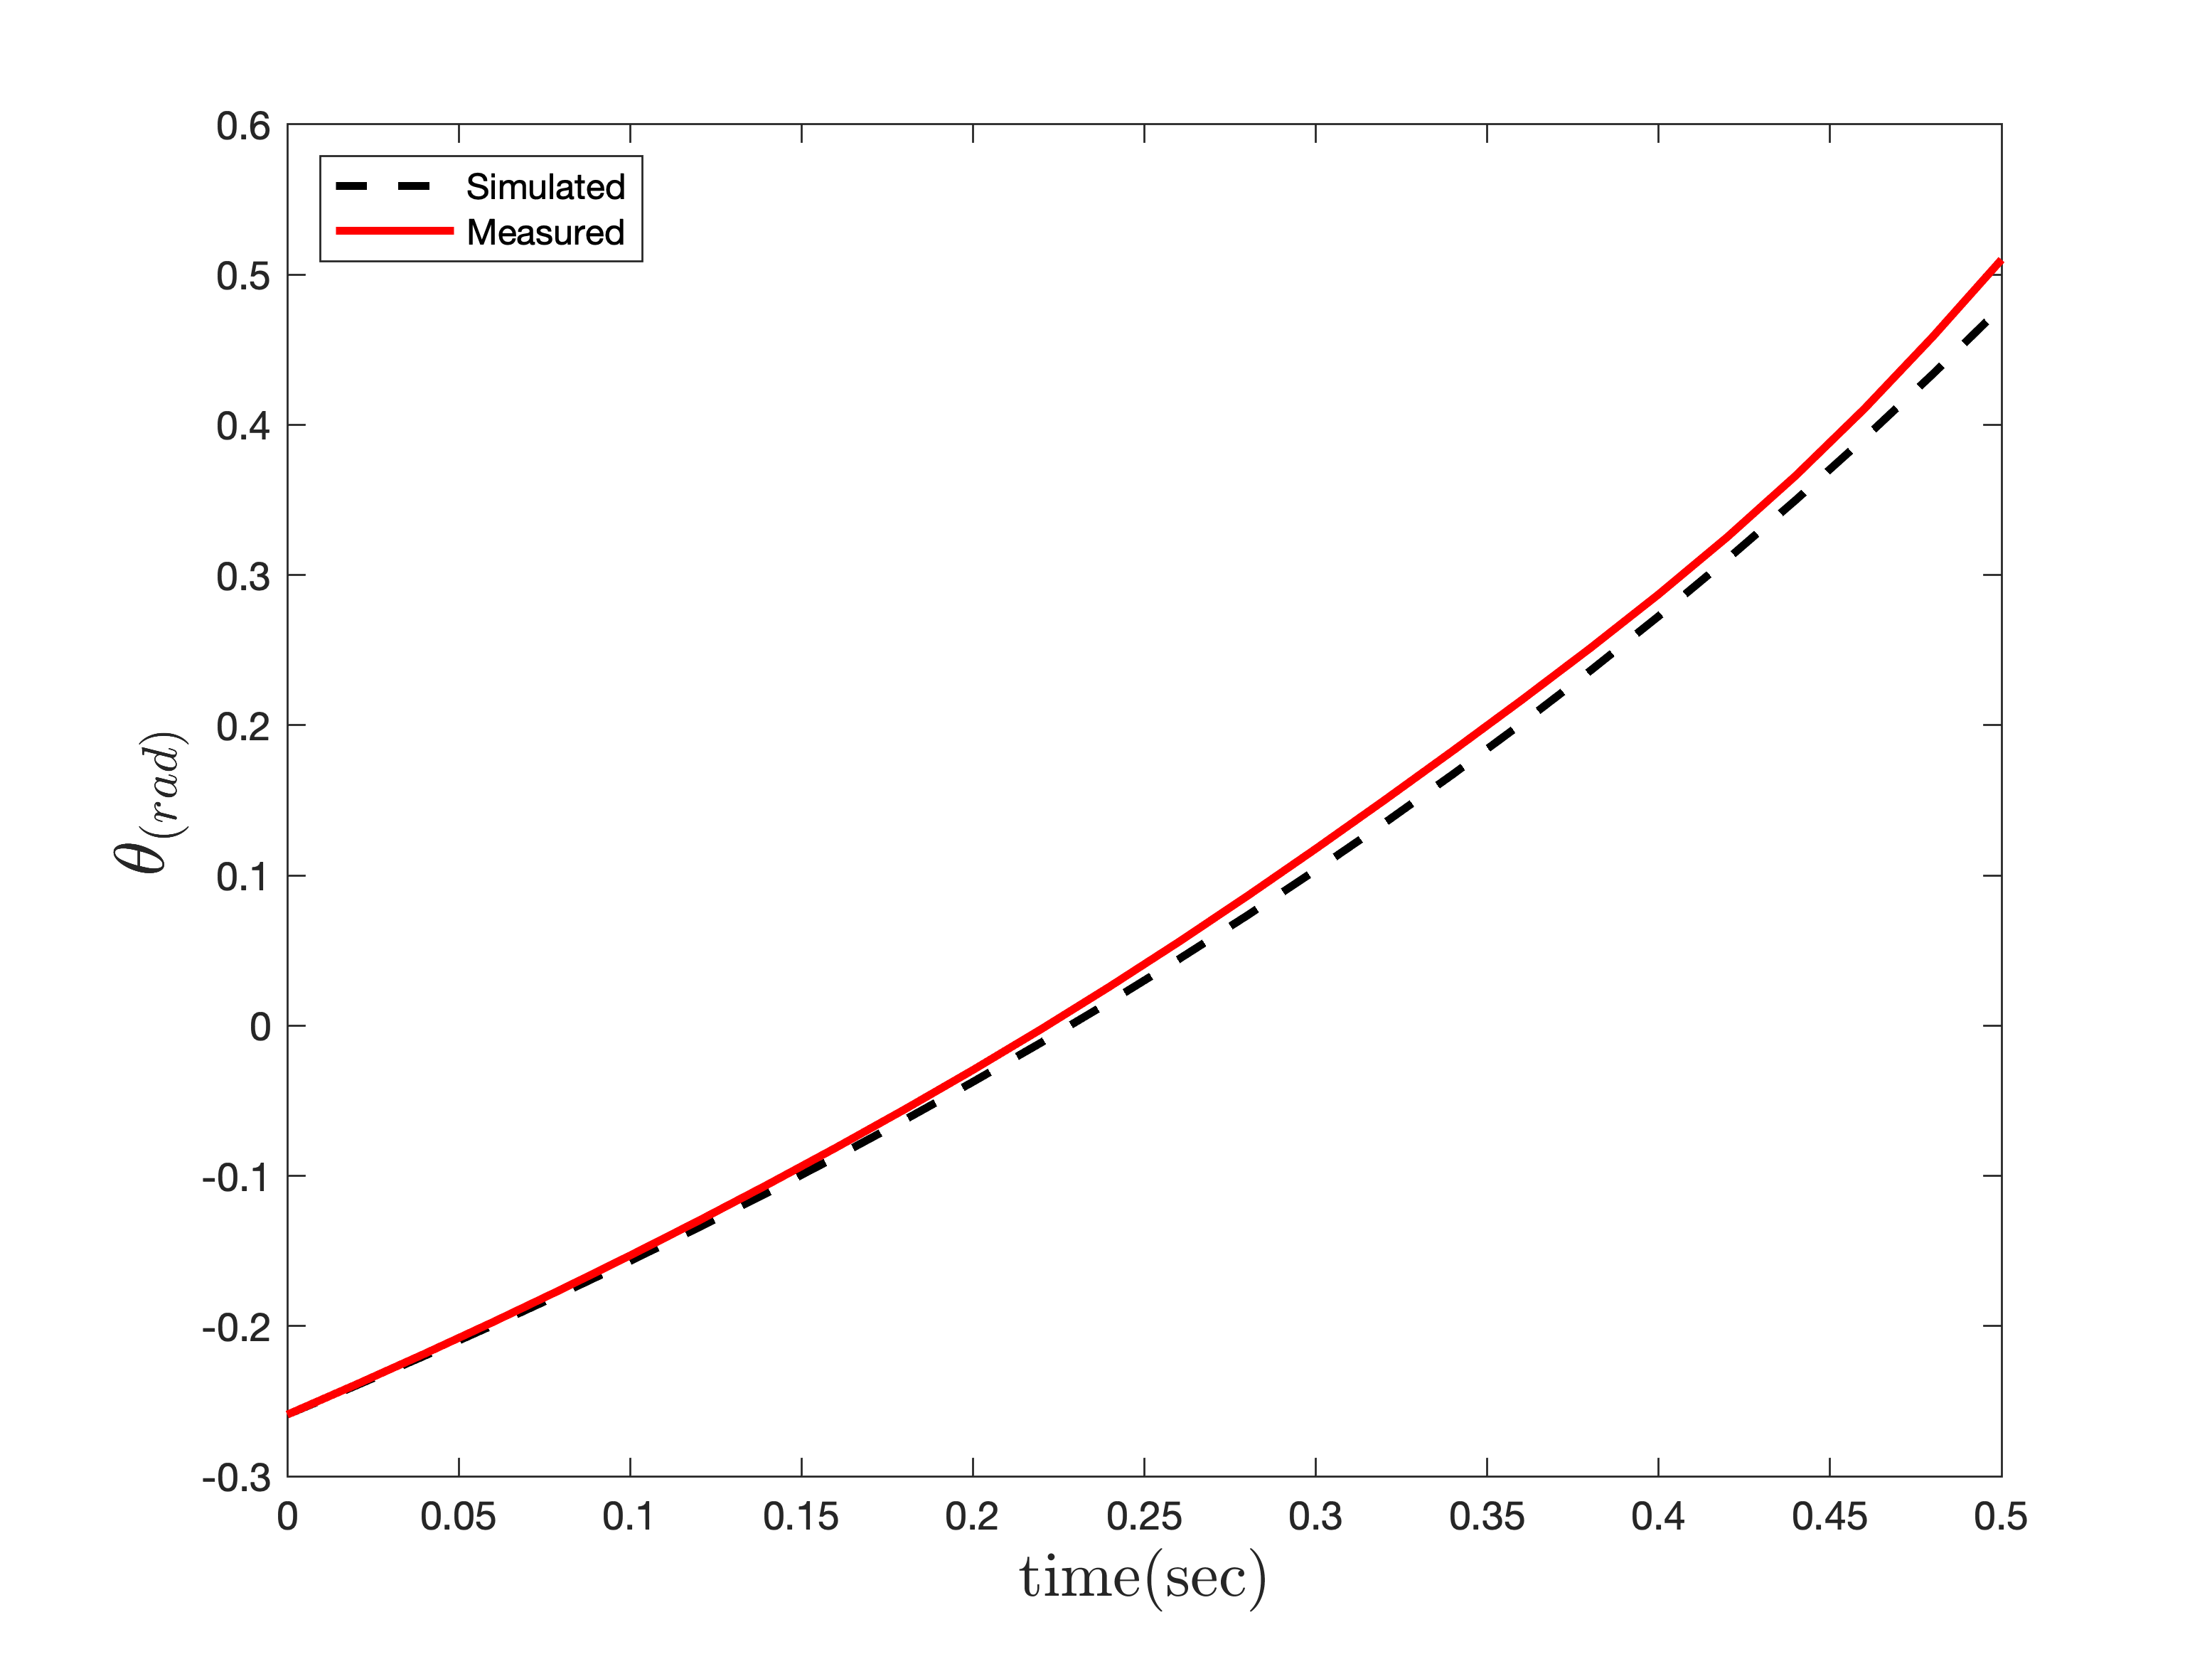
\includegraphics[width=.48\linewidth]{../Figures/RCP/pitch_parameter_estimation/RCP_pitch_S1.png}
%	\centering
%	\caption{مقايسه وضعیت استند در  آزمايش اول و شبیه‌سازی، پس از تخمین پارامترهای کانال پپچ}
%	\label{pitch_ps1}
%\end{figure}
%\begin{figure}[H]
%	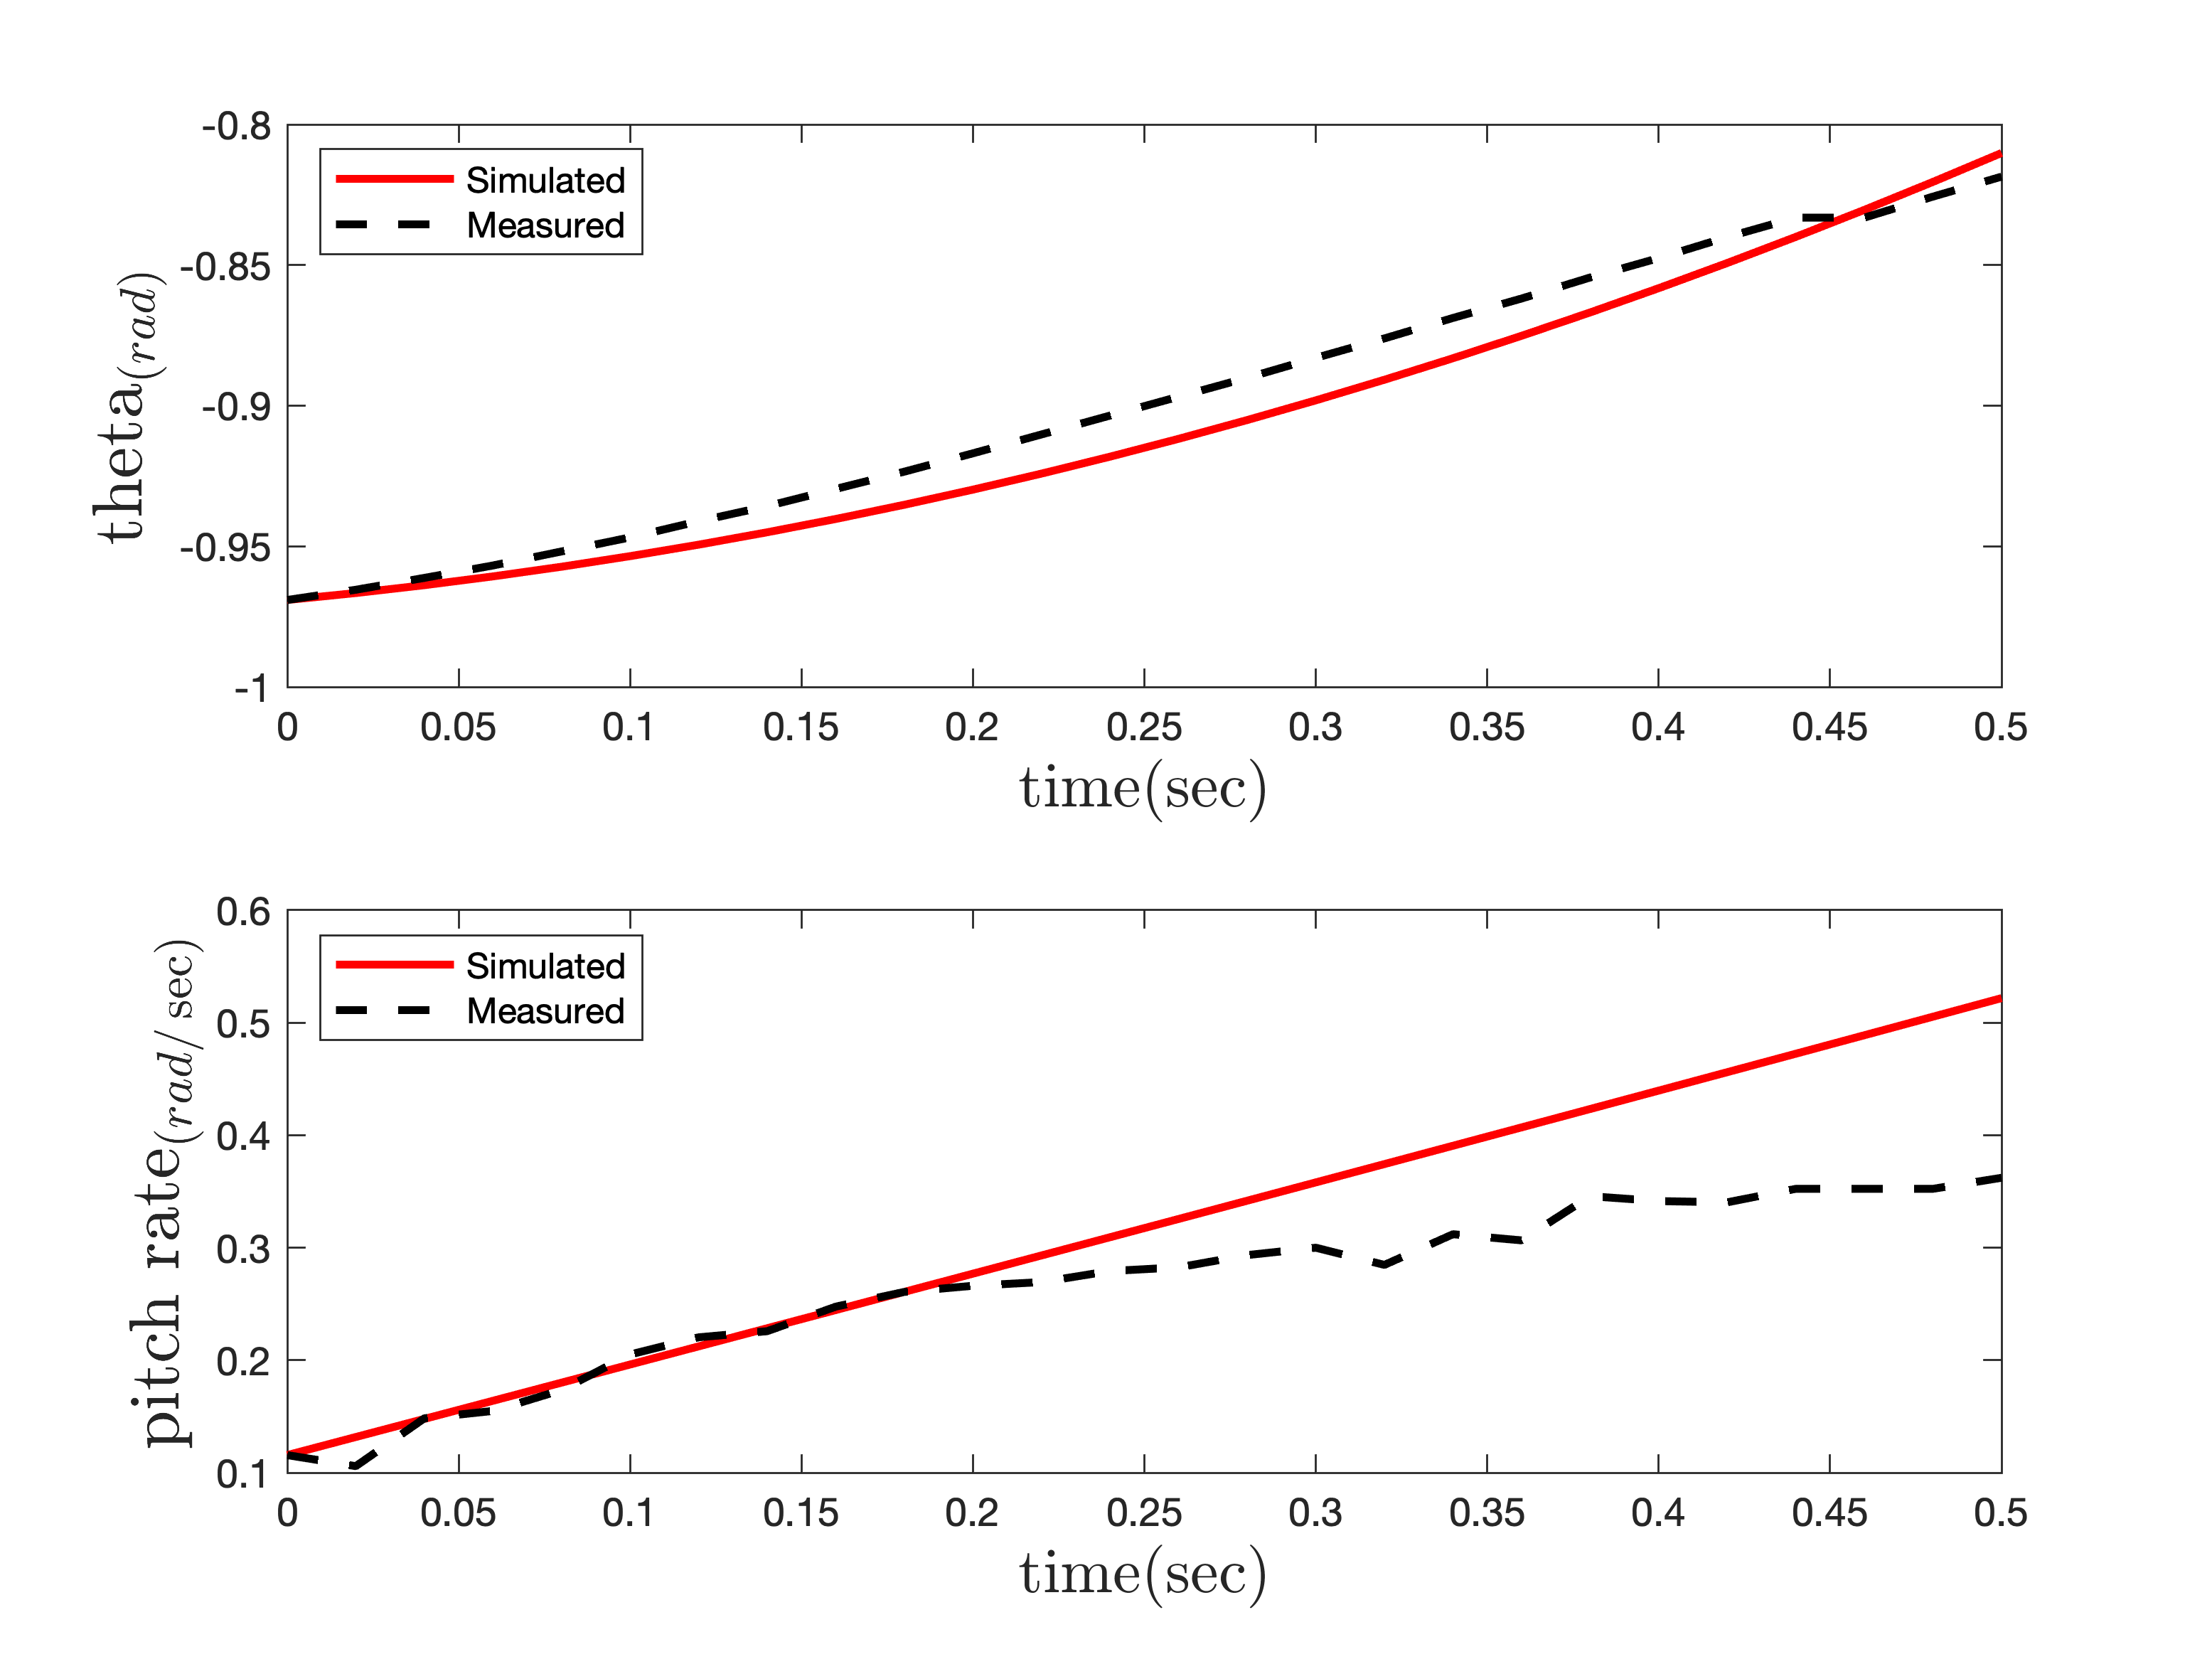
\includegraphics[width=12cm]{../Figures/RCP/pitch_parameter_estimation/RCP_pitch_S2.png}
%	\centering
%	\caption{مقايسه وضعیت استند در  آزمايش دوم و شبیه‌سازی، پس از تخمین پارامترهای کانال پپچ}
%	\label{pitch_ps2}
%\end{figure}
%\begin{figure}[H]
%	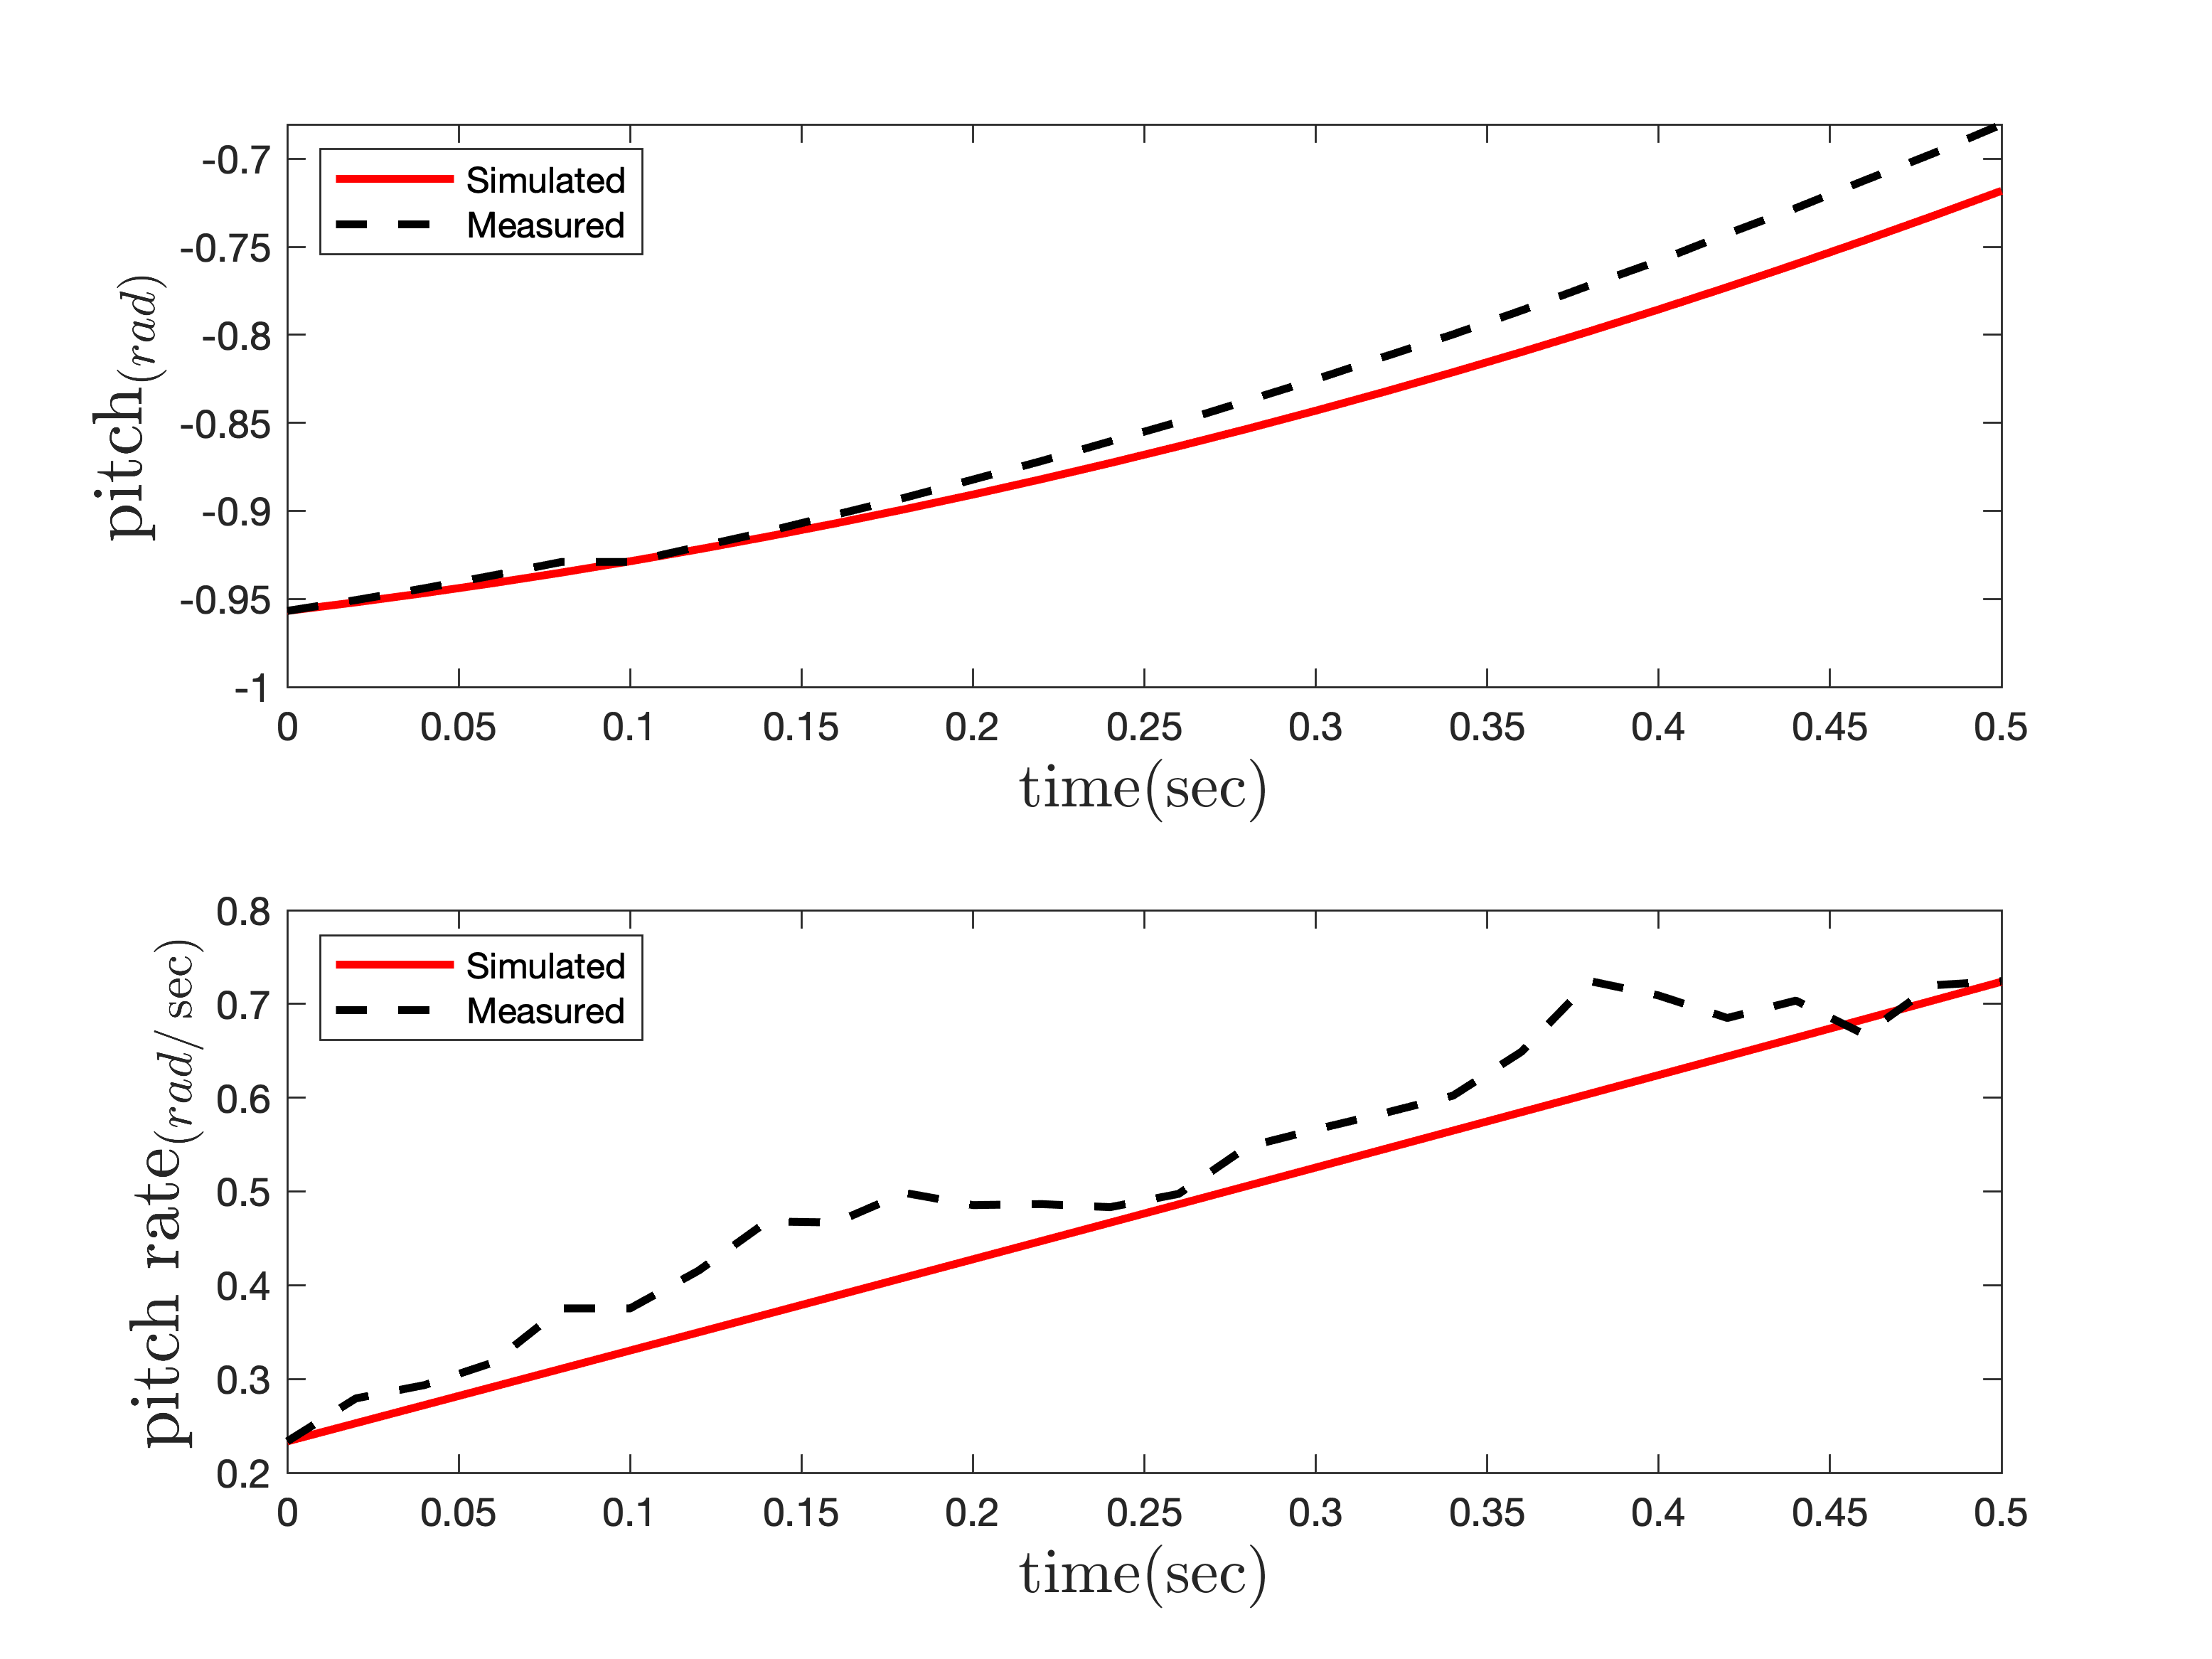
\includegraphics[width=12cm]{../Figures/RCP/pitch_parameter_estimation/RCP_pitch_S3.png}
%	\centering
%	\caption{مقايسه وضعیت استند در  آزمايش سوم و شبیه‌سازی، پس از تخمین پارامترهای کانال پپچ}
%	\label{pitch_ps3}
%\end{figure}
